\documentclass[aspectratio=169]{beamer}
\usetheme{Madrid}
\usecolortheme{default}

% Packages
\usepackage{graphicx}
\usepackage{booktabs}
\usepackage{array}
\usepackage{multirow}
\usepackage{algorithmic}
\usepackage{algorithm}
\usepackage{xcolor}
\usepackage{tikz}
\usetikzlibrary{shapes.geometric, arrows.meta, positioning}

\setbeamertemplate{navigation symbols}{}

% ── Footer (identical to template) ───────────────────────────────────
\setbeamertemplate{footline}{
    \leavevmode%
    \hbox{%
        \begin{beamercolorbox}[wd=.33\paperwidth,ht=2.5ex,dp=1ex,leftskip=1em]{author in head/foot}%
            \textbf{MNIT Jaipur}
        \end{beamercolorbox}%
        \begin{beamercolorbox}[wd=.33\paperwidth,ht=2.5ex,dp=1ex,center]{title in head/foot}%
            Minor Project
        \end{beamercolorbox}%
        \begin{beamercolorbox}[wd=.33\paperwidth,ht=2.5ex,dp=1ex,rightskip=1em]{date in head/foot}%
            November 2026 \hfill \insertframenumber/\inserttotalframenumber
        \end{beamercolorbox}%
    }%
    \vskip0pt%
}

% ── Title / Author / Institute (identical pattern to template) ────────
\title[Security \& Privacy Analysis of Preinstalled Android Apps]{%
    Security and Privacy Analysis of Preinstalled Android Applications
    Using Static Taint Analysis}

\author{\textbf{\textcolor{blue}{Kavyansh Tyagi}} (2022UCS1570)}

\institute{
    Malaviya National Institute of Technology, Jaipur \\
    Department of Computer Science and Engineering
    \\
}
\date{November 2026}
\vspace{2mm}


% ════════════════════════════════════════════════════════════════════
\begin{document}
% ════════════════════════════════════════════════════════════════════


%% ─────────────────────────────────────────────────────────────────
%% SLIDE 1 — Title Slide
%% ─────────────────────────────────────────────────────────────────
\begin{frame}
    \titlepage
    \vspace{-0.7cm}
    \begin{center}
        
\includegraphics[width=0.08\textwidth]{Mnit_logo.png}\\
        \small{Under the supervision of}\\
        \textbf{\textcolor{blue}{Dr.\ [Supervisor Name]}}, Assistant Professor
    \end{center}
\end{frame}


%% ─────────────────────────────────────────────────────────────────
%% Outline (not counted in 20 slides — acts as roadmap)
%% ─────────────────────────────────────────────────────────────────
\begin{frame}{Outline}
    \begin{itemize}
        \item Introduction
        \item Motivation
        \item Problem Statement
        \item Literature Review
        \item Research Gaps
        \item Objective
        \item Proposed Methodology
        \item Conclusion and Future Scope
        \item Acknowledgements
        \item References
    \end{itemize}
\end{frame}


%% ─────────────────────────────────────────────────────────────────
%% SLIDE 2 — Introduction I : Android Architecture
%% ─────────────────────────────────────────────────────────────────
\begin{frame}{Introduction}
\begin{columns}[T]
    \begin{column}{0.46\textwidth}
        \textbf{\textcolor{blue}{Android Architecture}}
        \vspace{4pt}

        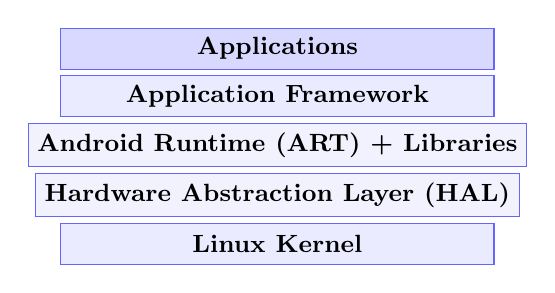
\begin{tikzpicture}[node distance=2pt]
            \tikzstyle{layer}=[rectangle, draw=blue!60, fill=blue!15,
                               minimum width=5.5cm, minimum height=0.52cm,
                               font=\small\bfseries, align=center]
            \tikzstyle{layer2}=[layer, fill=blue!8]
            \tikzstyle{layer3}=[layer, fill=blue!5]
            \node[layer]  (l1) {Applications};
            \node[layer2, below=of l1] (l2) {Application Framework};
            \node[layer3, below=of l2] (l3) {Android Runtime (ART) + Libraries};
            \node[layer3, below=of l3] (l4) {Hardware Abstraction Layer (HAL)};
            \node[layer2, below=of l4] (l5) {Linux Kernel};
        \end{tikzpicture}

        \vspace{6pt}
        \footnotesize
        \textit{Preinstalled apps reside in read-only partitions:
        \texttt{/system/app} and \texttt{/system/priv-app}.}
    \end{column}

    \begin{column}{0.52\textwidth}
        \textbf{\textcolor{blue}{Android Ecosystem}}
        \begin{itemize}
            \item Android powers \textbf{$\sim$72\%} of global mobile devices
            \item Over \textbf{3.5 billion} active Android devices worldwide
            \item Apps packaged as \textbf{APK} (Android Package Kit) files
            \item APK contains compiled \textbf{Dalvik/ART bytecode},
                  resources, and manifest
            \item \texttt{AndroidManifest.xml} declares permissions, components,
                  and intents
            \item Apps isolated via \textbf{UID-based} Linux process sandboxing
            \item Inter-process communication via \textbf{Binder IPC} mechanism
        \end{itemize}
    \end{column}
\end{columns}
\end{frame}


%% ─────────────────────────────────────────────────────────────────
%% SLIDE 3 — Introduction II : Preinstalled & System Apps
%% ─────────────────────────────────────────────────────────────────
\begin{frame}{Introduction}
\begin{columns}[T]
    \begin{column}{0.32\textwidth}
        \textbf{\textcolor{blue}{Preinstalled Applications}}
        \begin{itemize}
            \item Shipped with device firmware by OEM / carrier
            \item Stored in read-only \texttt{/system/app} partition
            \item Cannot be uninstalled without root access
            \item Include: Browser, Camera, Dialer, Messages, Maps
            \item Samsung-specific: Samsung Health, SmartThings, Bixby
        \end{itemize}
    \end{column}

    \begin{column}{0.32\textwidth}
        \textbf{\textcolor{blue}{System / Privileged Apps}}
        \begin{itemize}
            \item Located in \texttt{/system/priv-app}
            \item Declared with \texttt{signatureOrSystem} permissions
            \item Can bypass certain Android permission restrictions
            \item Access: telephony, location, contacts, storage
            \item Examples: Phone, Settings, System UI, PackageInstaller
        \end{itemize}
    \end{column}

    \begin{column}{0.32\textwidth}
        \textbf{\textcolor{blue}{Sensitive Resource Access}}
        \begin{itemize}
            \item Location (GPS, Network-based)
            \item Microphone and Camera
            \item Contacts, Call Logs, SMS / MMS
            \item Device identifiers (IMEI, IMSI, Android ID)
            \item Clipboard, Notifications, Accounts
        \end{itemize}
    \end{column}
\end{columns}

\vspace{8pt}
\begin{block}{}
\small
System-level apps inherit higher trust and broader resource access than
user-installed apps, yet receive comparatively little independent security scrutiny.
\end{block}
\end{frame}


%% ─────────────────────────────────────────────────────────────────
%% SLIDE 4 — Motivation
%% ─────────────────────────────────────────────────────────────────
\begin{frame}{Motivation}
\begin{itemize}
    \item \textbf{Invisible Attack Surface:}
          Preinstalled apps are present on every device of a given firmware,
          creating a uniform large-scale attack surface affecting millions of users.

    \item \textbf{Elevated Permissions by Default:}
          System apps often hold dangerous permissions
          (\texttt{READ\_CONTACTS}, \texttt{ACCESS\_FINE\_LOCATION},
          \texttt{READ\_CALL\_LOG}) without requiring runtime user consent,
          effectively bypassing Android's permission model.

    \item \textbf{Potential for Data Leakage:}
          Sensitive data (IMEI, location, messages, credentials) can flow from
          sensitive \textit{sources} to network sinks, files, or logs without user
          awareness — a classic \textbf{taint flow} scenario.

    \item \textbf{Lack of User Control:}
          Unlike third-party apps, users cannot uninstall or audit preinstalled
          apps, making proactive \textbf{static analysis} the primary defense
          mechanism available to researchers.

    \item \textbf{Prior Research Evidence:}
          Studies such as \textbf{FIRMSCOPE} (2020) and \textbf{An Analysis of
          Pre-installed Android Software} (2020) have demonstrated privilege-escalation
          vulnerabilities and undisclosed data-sharing behaviours in OEM firmware at scale.
\end{itemize}
\end{frame}


%% ─────────────────────────────────────────────────────────────────
%% SLIDE 5 — Problem Statement
%% ─────────────────────────────────────────────────────────────────
\begin{frame}{Problem Statement}

Preinstalled Android applications — bundled by OEMs such as Samsung —
possess elevated system-level permissions and access to sensitive device
resources. Identifying whether sensitive data flows from \textbf{privacy-sensitive
sources} to \textbf{potentially dangerous sinks} in these applications requires
systematic static taint analysis, which remains challenging due to:

\vspace{6pt}
\begin{itemize}
    \item \textbf{Scale:} Firmware images contain hundreds of preinstalled APKs,
          making exhaustive manual analysis infeasible.

    \item \textbf{Obfuscation:} OEM apps often apply code obfuscation, complicating
          static analysis and taint propagation tracking.

    \item \textbf{False Positives:} Static taint tools such as FlowDroid are known
          to produce false positive flows that require manual validation.

    \item \textbf{API Complexity:} Android provides hundreds of sensitive APIs;
          correct modeling of sources and sinks is critical for analysis accuracy.

    \item \textbf{Closed Source:} Preinstalled APKs ship without source code,
          requiring decompilation before any code-level analysis can be performed.
\end{itemize}
\end{frame}


%% ─────────────────────────────────────────────────────────────────
%% SLIDE 6 — Literature Review I
%% ─────────────────────────────────────────────────────────────────
\begin{frame}{Literature Review I}
\begin{table}[ht]
    \centering
    \caption{Related Work — Firmware \& Pre-installed App Analysis}
    \tiny
    \begin{tabular}{|p{0.6in}|p{0.65in}|p{1.0in}|p{1.3in}|p{1.3in}|}
    \hline
    \textbf{Paper} & \textbf{Authors / Year} & \textbf{Objective} &
    \textbf{Contributions} & \textbf{Limitations} \\
    \hline
    \vspace{1mm}
    FIRMSCOPE &
    Almakhdhub et al., USENIX 2020 &
    Discover privilege-escalation vulnerabilities in pre-installed apps across OEM firmware &
    \begin{itemize}
        \item Found 850+ exploitable vulnerabilities across 2,017 firmware images from 11 OEMs
        \item Proposed Monodroid-based scalable analysis pipeline
    \end{itemize} &
    \begin{itemize}
        \item High false-positive rate
        \item Does not cover runtime or dynamic flows
    \end{itemize} \\
    \hline
    \vspace{1mm}
    An Analysis of Pre-installed Android Software &
    Gamba et al., IEEE S\&P 2020 &
    Characterise data collection and sharing behaviour of pre-installed software at scale &
    \begin{itemize}
        \item Identified 4,845 apps with potential privacy-sensitive behaviours
        \item Found undisclosed third-party data sharing across 1,742 firmware images
    \end{itemize} &
    \begin{itemize}
        \item Limited to network-observable flows
        \item Encrypted traffic limits analysis completeness
    \end{itemize} \\
    \hline
    \end{tabular}
\end{table}
\end{frame}


%% ─────────────────────────────────────────────────────────────────
%% SLIDE 7 — Literature Review II
%% ─────────────────────────────────────────────────────────────────
\begin{frame}{Literature Review II}
\begin{table}[ht]
    \centering
    \caption{Related Work — Hybrid Analysis \& EU OEM Data Flows}
    \tiny
    \begin{tabular}{|p{0.6in}|p{0.65in}|p{1.0in}|p{1.3in}|p{1.3in}|}
    \hline
    \textbf{Paper} & \textbf{Authors / Year} & \textbf{Objective} &
    \textbf{Contributions} & \textbf{Limitations} \\
    \hline
    \vspace{1mm}
    DroidRay &
    Wong \& Lie, ASIACCS 2014 &
    Detect privacy leaks in Android apps by combining static and dynamic taint analysis &
    \begin{itemize}
        \item Reduced false positives compared to pure static tools
        \item Prototype evaluated on 1,500+ apps
    \end{itemize} &
    \begin{itemize}
        \item High overhead in dynamic tracing
        \item Requires device execution; limited to observed paths
    \end{itemize} \\
    \hline
    \vspace{1mm}
    ``Do Android Dream of Electric Sheep?'' &
    Kunze et al., PoPETS 2022 &
    Assess data flows in OEM-bundled Android apps across EU smartphone brands &
    \begin{itemize}
        \item Found persistent device identifiers sent without user consent
        \item Raised GDPR compliance concerns for Samsung, Xiaomi, Realme
    \end{itemize} &
    \begin{itemize}
        \item Coverage limited to network-observable flows
        \item Encrypted HTTPS traffic could not be fully decoded
    \end{itemize} \\
    \hline
    \end{tabular}
\end{table}
\end{frame}


%% ─────────────────────────────────────────────────────────────────
%% SLIDE 8 — Literature Review III
%% ─────────────────────────────────────────────────────────────────
\begin{frame}{Literature Review III}
\begin{table}[ht]
    \centering
    \caption{Related Work — Low-Cost Devices \& Bloatware Taxonomy}
    \tiny
    \begin{tabular}{|p{0.6in}|p{0.65in}|p{1.0in}|p{1.3in}|p{1.3in}|}
    \hline
    \textbf{Paper} & \textbf{Authors / Year} & \textbf{Objective} &
    \textbf{Contributions} & \textbf{Limitations} \\
    \hline
    \vspace{1mm}
    PiPLAnD &
    Reyes et al., WPES &
    Examine security \& privacy of pre-installed apps in budget Android devices targeting developing markets &
    \begin{itemize}
        \item Found widespread misuse of dangerous permissions
        \item Identified apps tracking users without disclosure
    \end{itemize} &
    \begin{itemize}
        \item Limited to manifest-level and partial code inspection
        \item No full taint-flow analysis performed
    \end{itemize} \\
    \hline
    \vspace{1mm}
    Pleasure or Pain? &
    Zhan et al., IEEE TDSC 2020 &
    Evaluate the costs (security, privacy, performance) and utilities of bloatware in Android smartphones &
    \begin{itemize}
        \item Established a taxonomy of bloatware
        \item Showed negative user-experience and security risks from pre-installed apps
    \end{itemize} &
    \begin{itemize}
        \item No deep taint analysis performed
        \item Relies on user survey and manifest-level static checks only
    \end{itemize} \\
    \hline
    \end{tabular}
\end{table}
\end{frame}


%% ─────────────────────────────────────────────────────────────────
%% SLIDE 9 — Literature Review IV
%% ─────────────────────────────────────────────────────────────────
\begin{frame}{Literature Review IV}
\begin{table}[ht]
    \centering
    \caption{Related Work — Static Taint Analysis Tools}
    \tiny
    \begin{tabular}{|p{0.6in}|p{0.65in}|p{1.0in}|p{1.3in}|p{1.3in}|}
    \hline
    \textbf{Paper} & \textbf{Authors / Year} & \textbf{Objective} &
    \textbf{Contributions} & \textbf{Limitations} \\
    \hline
    \vspace{1mm}
    FlowDroid &
    Arzt et al., ACM PLDI 2014 &
    Provide precise, context-, flow-, field- and object-sensitive static taint analysis for Android &
    \begin{itemize}
        \item Gold-standard taint analysis tool for Android
        \item Open-source; used in dozens of subsequent research studies
        \item Lifecycle-aware Android model (Activity, Service)
    \end{itemize} &
    \begin{itemize}
        \item Scalability issues on large apps
        \item Reflective calls not fully modeled
    \end{itemize} \\
    \hline
    \vspace{1mm}
    AndroidLeaks &
    Gibler et al., TRUST 2012 &
    Automatically detect personal information leaks in Android apps using static analysis &
    \begin{itemize}
        \item One of the earliest large-scale static leak detection systems
        \item Tested on 1,000+ Android apps
    \end{itemize} &
    \begin{itemize}
        \item Lacks context sensitivity
        \item Limited source/sink coverage vs.\ later tools
    \end{itemize} \\
    \hline
    \end{tabular}
\end{table}
\end{frame}


%% ─────────────────────────────────────────────────────────────────
%% SLIDE 10 — Literature Review V
%% ─────────────────────────────────────────────────────────────────
\begin{frame}{Literature Review V}
\begin{table}[ht]
    \centering
    \caption{Related Work — General Android Analysis Frameworks}
    \tiny
    \begin{tabular}{|p{0.6in}|p{0.65in}|p{1.0in}|p{1.3in}|p{1.3in}|}
    \hline
    \textbf{Paper} & \textbf{Authors / Year} & \textbf{Objective} &
    \textbf{Contributions} & \textbf{Limitations} \\
    \hline
    \vspace{1mm}
    Amandroid &
    Wei et al., ACM CCS 2014 &
    Build a general Android security analysis framework supporting inter-component communication (ICC) &
    \begin{itemize}
        \item Handles component-to-component flows via Intent resolution
        \item More comprehensive than FlowDroid for multi-component apps
    \end{itemize} &
    \begin{itemize}
        \item Higher analysis time due to ICC modeling
        \item Some underapproximation of reflection
    \end{itemize} \\
    \hline
    \vspace{1mm}
    DroidSafe &
    Gordon et al., NDSS 2015 &
    Provide sound information-flow analysis for Android apps with accurate Android API modeling &
    \begin{itemize}
        \item More precise Android API semantics than FlowDroid
        \item Reduced false negatives in source/sink modeling via Android Test Environment (ATE)
    \end{itemize} &
    \begin{itemize}
        \item Very high analysis time
        \item ATE construction requires significant engineering effort
    \end{itemize} \\
    \hline
    \end{tabular}
\end{table}
\end{frame}


%% ─────────────────────────────────────────────────────────────────
%% SLIDE 11 — Research Gaps
%% ─────────────────────────────────────────────────────────────────
\begin{frame}{Research Gaps}
\begin{itemize}
    \item \textbf{Firmware-Level vs.\ Device-Specific Analysis:}
          Most studies (FIRMSCOPE, Gamba et al.) analyse bulk firmware datasets and do not
          perform in-depth, device-specific analysis. A focused study of a single OEM device
          (e.g., Samsung) can produce more actionable, targeted findings.

    \item \textbf{Limited Use of Precision Taint Analysis:}
          Several papers rely on manifest inspection or traffic analysis rather than full
          inter-procedural, field-sensitive taint analysis. Tools such as FlowDroid enable
          precise source-to-sink tracking that most large-scale studies forgo.

    \item \textbf{False Positive Validation Absent:}
          Existing studies often report potential flows without systematic validation of false
          positives. A rigorous manual review of flagged flows is needed to confirm real leakage risks.

    \item \textbf{Samsung Ecosystem Underrepresented:}
          Samsung is the world's largest Android OEM, yet device-specific static taint analysis
          of Samsung One UI / preinstalled apps remains limited in published literature.

    \item \textbf{Toolchain Integration Gap:}
          No study combines APK extraction via \textbf{ADB}, decompilation via
          \textbf{JADX/Apktool}, and \textbf{FlowDroid} taint analysis into a single
          reproducible, documented open-source workflow for a specific OEM device.
\end{itemize}
\end{frame}


%% ─────────────────────────────────────────────────────────────────
%% SLIDE 12 — Objective I : Main + Specific Objectives
%% ─────────────────────────────────────────────────────────────────
\begin{frame}{Objective}

\textbf{\textcolor{blue}{Main Objective:}}\\[4pt]
To perform a systematic \textbf{static taint analysis} of preinstalled Android applications
on a Samsung device in order to identify potential sensitive data flows from privacy-sensitive
sources to potentially dangerous sinks, and to document the findings in a structured,
reproducible analysis report.

\vspace{8pt}
\textbf{\textcolor{blue}{Specific Objectives:}}
\begin{itemize}
    \item \textbf{SO1:} Extract and catalogue preinstalled APKs from a Samsung Android device
          using ADB.
    \item \textbf{SO2:} Select a representative subset of apps based on declared permissions
          and system functionality.
    \item \textbf{SO3:} Decompile and statically inspect selected APKs using JADX and Apktool
          to understand code structure and permission usage.
    \item \textbf{SO4:} Apply FlowDroid to perform precise, inter-procedural source-to-sink
          taint flow analysis on each selected APK.
    \item \textbf{SO5:} Validate detected flows, assess false positives and document findings
          in a reproducible analysis report.
\end{itemize}
\end{frame}


%% ─────────────────────────────────────────────────────────────────
%% SLIDE 13 — Objective II : Research Questions & Contributions
%% ─────────────────────────────────────────────────────────────────
\begin{frame}{Objective}
\begin{columns}[T]
    \begin{column}{0.48\textwidth}
        \textbf{\textcolor{blue}{Research Questions}}
        \begin{itemize}
            \item \textbf{RQ1:} Which preinstalled Samsung apps declare and
                  use \textbf{dangerous permissions}?

            \item \textbf{RQ2:} Do any apps contain identifiable
                  \textbf{source-to-sink data flows} involving sensitive APIs?

            \item \textbf{RQ3:} What categories of sensitive sources and sinks
                  are most prevalent in preinstalled apps?

            \item \textbf{RQ4:} How many detected flows can be confirmed as
                  \textbf{true positives} after manual validation?
        \end{itemize}
    \end{column}

    \begin{column}{0.48\textwidth}
        \textbf{\textcolor{blue}{Expected Contributions}}
        \begin{itemize}
            \item A curated dataset of preinstalled Samsung APKs with
                  permission metadata
            \item List of apps with dangerous permission declarations
            \item Classified source-to-sink taint flows per app
            \item Assessment of false positive rate and validation methodology
            \item Reproducible, documented analysis workflow using
                  open-source tools
            \item Structured academic report suitable for peer review
        \end{itemize}
    \end{column}
\end{columns}
\end{frame}


%% ─────────────────────────────────────────────────────────────────
%% SLIDE 14 — Proposed Methodology I : Workflow Overview
%% ─────────────────────────────────────────────────────────────────
\begin{frame}{Proposed Methodology}

\begin{figure}
    \centering
    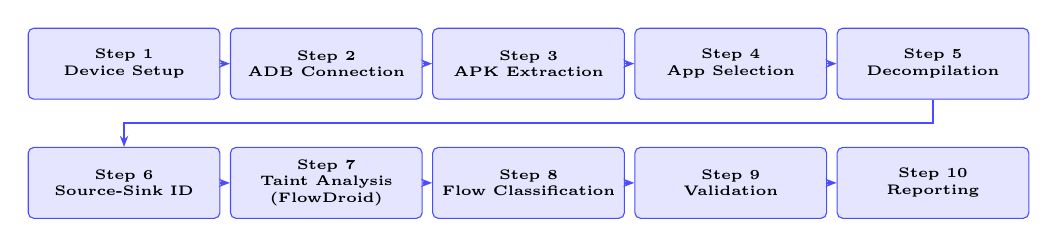
\begin{tikzpicture}[
        node distance = 0.28cm and 0.12cm,
        box/.style = {rectangle, draw=blue!70, fill=blue!10, rounded corners=2pt,
                      minimum width=2.3cm, minimum height=0.9cm,
                      font=\tiny\bfseries, align=center, text width=2.2cm},
        arr/.style = {-{Stealth[length=4pt]}, blue!70, line width=0.6pt}
    ]
        \node[box] (s1) {Step 1\\Device Setup};
        \node[box, right=of s1] (s2) {Step 2\\ADB Connection};
        \node[box, right=of s2] (s3) {Step 3\\APK Extraction};
        \node[box, right=of s3] (s4) {Step 4\\App Selection};
        \node[box, right=of s4] (s5) {Step 5\\Decompilation};

        \node[box, below=0.6cm of s1] (s6) {Step 6\\Source-Sink ID};
        \node[box, right=of s6] (s7) {Step 7\\Taint Analysis\\(FlowDroid)};
        \node[box, right=of s7] (s8) {Step 8\\Flow Classification};
        \node[box, right=of s8] (s9) {Step 9\\Validation};
        \node[box, right=of s9] (s10){Step 10\\Reporting};

        \draw[arr] (s1)--(s2); \draw[arr] (s2)--(s3);
        \draw[arr] (s3)--(s4); \draw[arr] (s4)--(s5);
        \draw[arr] (s5.south) -- ++(0,-0.3) -| (s6.north);
        \draw[arr] (s6)--(s7); \draw[arr] (s7)--(s8);
        \draw[arr] (s8)--(s9); \draw[arr] (s9)--(s10);
    \end{tikzpicture}
    \caption{Planned 10-Step Methodology Workflow}
\end{figure}

\vspace{2pt}
\begin{columns}[T]
    \begin{column}{0.48\textwidth}
        \textbf{\textcolor{blue}{Phase 1 — Setup \& Preparation (Steps 1–5)}}\\
        \footnotesize
        Device configuration, APK extraction via ADB, app selection based on
        dangerous permissions, and static decompilation using JADX / Apktool.
    \end{column}
    \begin{column}{0.48\textwidth}
        \textbf{\textcolor{blue}{Phase 2 — Analysis \& Reporting (Steps 6–10)}}\\
        \footnotesize
        Source/sink identification, FlowDroid taint analysis, flow classification,
        manual validation of false positives, and structured documentation.
    \end{column}
\end{columns}
\end{frame}


%% ─────────────────────────────────────────────────────────────────
%% SLIDE 15 — Proposed Methodology II : Tool Stack
%% ─────────────────────────────────────────────────────────────────
\begin{frame}{Proposed Methodology}
\begin{table}[ht]
    \centering
    \caption{Planned Tool Stack}
    \tiny
    \begin{tabular}{|p{0.9in}|p{1.2in}|p{2.0in}|p{1.5in}|}
    \hline
    \textbf{Tool} & \textbf{Purpose} & \textbf{Key Planned Operations} & \textbf{Output} \\
    \hline
    \vspace{1mm}
    \textbf{ADB} (Android Debug Bridge) &
    Device communication \& APK extraction &
    \texttt{adb shell pm list packages -f -s} \newline
    \texttt{adb pull /system/app/<App>.apk} &
    Raw APK files + metadata \\
    \hline
    \vspace{1mm}
    \textbf{JADX} &
    Decompile Dalvik $\rightarrow$ Java source &
    Browse class hierarchies, method bodies; identify API calls to sensitive sources/sinks &
    Java source code (read-only) for manual review \\
    \hline
    \vspace{1mm}
    \textbf{Apktool} &
    APK disassembly to Smali + manifest &
    Decode \texttt{AndroidManifest.xml}; inspect permissions, exported components &
    Smali bytecode, decoded manifest \\
    \hline
    \vspace{1mm}
    \textbf{FlowDroid} &
    Static taint analysis (IFDS / Soot) &
    Configure \texttt{SourcesAndSinks.txt}; run per-APK analysis; collect source $\rightarrow$ sink flow reports &
    Taint flow XML/JSON with call-chain evidence \\
    \hline
    \vspace{1mm}
    \textbf{MobSF} &
    Automated preliminary survey &
    Rapid permission risk scoring; certificate info; initial survey before focused FlowDroid analysis &
    HTML / JSON analysis report \\
    \hline
    \end{tabular}
\end{table}
\end{frame}


%% ─────────────────────────────────────────────────────────────────
%% SLIDE 16 — Proposed Methodology III : APK Extraction & Selection
%% ─────────────────────────────────────────────────────────────────
\begin{frame}{Proposed Methodology}
\begin{columns}[T]
    \begin{column}{0.48\textwidth}
        \textbf{\textcolor{blue}{Planned APK Extraction Steps}}
        \begin{enumerate}\small
            \item Enable Developer Options $\rightarrow$ USB Debugging on Samsung device
            \item Connect device via USB; authorize ADB host connection
            \item List system packages:\\
                  {\footnotesize\texttt{adb shell pm list packages -f -s}}
            \item Enumerate paths under \texttt{/system/app} and
                  \texttt{/system/priv-app}
            \item Pull APKs:\\
                  {\footnotesize\texttt{adb pull <remote\_path> <local\_dest>}}
            \item Verify APK integrity via SHA-256 checksum
            \item Record metadata: package name, version, partition,
                  permissions
        \end{enumerate}
    \end{column}

    \begin{column}{0.48\textwidth}
        \textbf{\textcolor{blue}{App Selection Criteria}}
        \begin{itemize}\small
            \item \textbf{Permission-Based:}
                  Declares $\geq$1 dangerous permission
                  (\texttt{ACCESS\_FINE\_LOCATION},
                  \texttt{READ\_CONTACTS},
                  \texttt{READ\_CALL\_LOG},
                  \texttt{RECORD\_AUDIO},
                  \texttt{READ\_SMS})

            \item \textbf{Functionality-Based:}
                  Communication apps (Phone, Messages, Email),
                  health/sensor apps (Samsung Health),
                  browser or WebView-based apps with network access

            \item \textbf{Priority Partitions:}
                  Apps in \texttt{/system/priv-app} (elevated privileges)
                  selected first; pre-grant permission holders prioritized

            \item \textbf{Exclusion Criteria:}
                  Apps declaring no dangerous permissions and with no
                  network access are deprioritized
        \end{itemize}
    \end{column}
\end{columns}
\end{frame}


%% ─────────────────────────────────────────────────────────────────
%% SLIDE 17 — Proposed Methodology IV : FlowDroid Pipeline & Sources/Sinks
%% ─────────────────────────────────────────────────────────────────
\begin{frame}{Proposed Methodology}

\begin{figure}
    \centering
    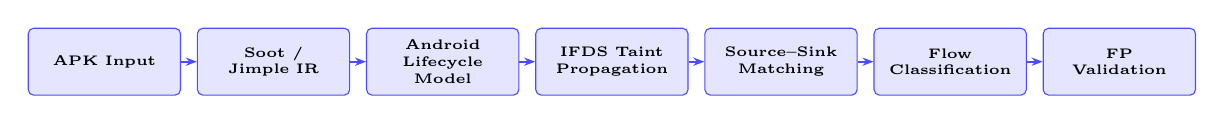
\begin{tikzpicture}[
        node distance = 0.2cm,
        box/.style = {rectangle, draw=blue!70, fill=blue!10, rounded corners=2pt,
                      minimum width=1.75cm, minimum height=0.85cm,
                      font=\tiny\bfseries, align=center, text width=1.7cm},
        arr/.style = {-{Stealth[length=4pt]}, blue!70, line width=0.6pt}
    ]
        \node[box] (a1) {APK Input};
        \node[box, right=of a1] (a2) {Soot /\\Jimple IR};
        \node[box, right=of a2] (a3) {Android\\Lifecycle\\Model};
        \node[box, right=of a3] (a4) {IFDS Taint\\Propagation};
        \node[box, right=of a4] (a5) {Source--Sink\\Matching};
        \node[box, right=of a5] (a6) {Flow\\Classification};
        \node[box, right=of a6] (a7) {FP\\Validation};

        \draw[arr](a1)--(a2); \draw[arr](a2)--(a3); \draw[arr](a3)--(a4);
        \draw[arr](a4)--(a5); \draw[arr](a5)--(a6); \draw[arr](a6)--(a7);
    \end{tikzpicture}
    \caption{Planned FlowDroid Static Taint Analysis Pipeline}
\end{figure}

\vspace{4pt}
\begin{columns}[T]
    \begin{column}{0.48\textwidth}
        \textbf{\textcolor{blue}{Planned Sensitive Sources}}
        \begin{itemize}\footnotesize
            \item \texttt{getLastKnownLocation()},
                  \texttt{requestLocationUpdates()}
            \item \texttt{TelephonyManager.getDeviceId()},
                  \texttt{getSubscriberId()}
            \item \texttt{ContentResolver} $\rightarrow$ Contacts, SMS, Call Log
            \item \texttt{AudioRecord.read()} (Microphone)
            \item \texttt{AccountManager.getAccounts()}
            \item \texttt{ClipboardManager.getPrimaryClip()}
        \end{itemize}
    \end{column}

    \begin{column}{0.48\textwidth}
        \textbf{\textcolor{blue}{Planned Dangerous Sinks}}
        \begin{itemize}\footnotesize
            \item Network I/O: \texttt{HttpURLConnection}, \texttt{OkHttp},
                  \texttt{Socket}
            \item File writes: \texttt{FileOutputStream},
                  \texttt{SharedPreferences}
            \item SMS sending APIs
            \item Logging: \texttt{Log.d()}, \texttt{Log.e()} with sensitive data
            \item Intent / IPC broadcasts with sensitive extras
            \item \texttt{ContentProvider} insert / update operations
        \end{itemize}
    \end{column}
\end{columns}
\end{frame}


%% ─────────────────────────────────────────────────────────────────
%% SLIDE 18 — Conclusion and Future Scope
%% ─────────────────────────────────────────────────────────────────
\begin{frame}{Conclusion and Future Scope}
\small
This research \textbf{proposes} a systematic static taint analysis of preinstalled
applications on a Samsung Android device. By combining APK extraction via ADB,
decompilation using JADX and Apktool, and precise taint flow analysis using FlowDroid,
the study \textit{aims} to identify and document potential sensitive data flows in
system-level apps that most users cannot remove or audit. Literature evidence confirms
that such analysis is both necessary and feasible at the per-device level.

\vspace{6pt}
\textbf{\textcolor{blue}{Expected Outcomes (Planned):}}
\begin{itemize}
    \item Catalogue of preinstalled Samsung APKs with permission metadata
    \item Identified potential source-to-sink taint flows per app
    \item Validated list of true-positive privacy-relevant flows after manual review
    \item Reproducible open-source analysis workflow documentation
\end{itemize}

\vspace{4pt}
\textbf{Future Work:}
\begin{itemize}
    \item Extend analysis to multiple Samsung firmware versions and other OEM devices
    \item Integrate dynamic taint tracking at runtime to complement static findings
    \item Automate the pipeline for continuous firmware-level security monitoring
    \item Compare cross-OEM findings and contribute to open source/sink databases
\end{itemize}
\end{frame}


%% ─────────────────────────────────────────────────────────────────
%% SLIDE 19 — Acknowledgements
%% ─────────────────────────────────────────────────────────────────
\begin{frame}{Acknowledgements}
\begin{itemize}
    \item We sincerely express our gratitude to
          \textbf{\textcolor{blue}{Dr.\ [Supervisor Name]}},
          Assistant Professor, Department of Computer Science and Engineering,
          MNIT Jaipur, for invaluable guidance, continuous feedback and academic
          mentorship throughout the planning and execution of this research proposal.

    \vspace{6pt}
    \item We thank the faculty members of the Department of Computer Science and
          Engineering, \textbf{Malaviya National Institute of Technology, Jaipur},
          for their constructive evaluation and academic support during the
          mid-evaluation process.

    \vspace{6pt}
    \item We express our gratitude to \textbf{MNIT Jaipur} for providing access to
          academic resources, library databases, laboratory infrastructure and a
          conducive research environment throughout the duration of this project.
\end{itemize}
\end{frame}


%% ─────────────────────────────────────────────────────────────────
%% SLIDE 20 — References
%% ─────────────────────────────────────────────────────────────────
\begin{frame}[allowframebreaks]{References}
\scriptsize
\begin{enumerate}
    \item N.\ Almakhdhub, A.\ Machiry, S.\ Rahimi, C.\ Kruegel, G.\ Vigna,
          ``FIRMSCOPE: Automatic Uncovering of Privilege-Escalation Vulnerabilities
          in Pre-Installed Apps in Android Firmware,''
          \textit{USENIX Security Symposium}, 2020.

    \item J.\ Gamba, M.\ Rashed, A.\ Razaghpanah, J.\ Tapiador, N.\ Vallina-Rodriguez,
          ``An Analysis of Pre-Installed Android Software,''
          \textit{IEEE Symposium on Security \& Privacy (S\&P)}, 2020.

    \item M.\ Wong, D.\ Lie,
          ``DroidRay: A Security Evaluation System for Customized Android Firmwares,''
          \textit{ACM ASIA Conference on Computer and Communications Security (ASIACCS)},
          2014.

    \item L.\ Kunze, N.\ Becker, K.\ Bhatt, T.\ Lauinger, A.\ Zareian,
          ``Do Android Dream of Electric Sheep?\ Analyzing Pre-installed Android Apps
          in the Wild,''
          \textit{Privacy Enhancing Technologies Symposium (PoPETS)}, 2022.

    \item I.\ Reyes et al.,
          ``PiPLAnD: On the Security of Pre-installed Android Apps in Low-cost Devices,''
          \textit{ACM Workshop on Privacy in the Electronic Society (WPES)}, 2018.

    \item X.\ Zhan et al.,
          ``Pleasure or Pain?\ An Evaluation of the Costs and Utilities of Bloatware
          Applications in Android Smartphones,''
          \textit{IEEE Transactions on Dependable and Secure Computing}, 2020.

    \item S.\ Arzt, S.\ Rasthofer, C.\ Fritz, E.\ Bodden et al.,
          ``FlowDroid: Precise Context, Flow, Field, Object-Sensitive and
          Lifecycle-Aware Taint Analysis for Android Apps,''
          \textit{ACM SIGPLAN PLDI}, 2014.

    \item C.\ Gibler, J.\ Crussell, J.\ Erickson, H.\ Chen,
          ``AndroidLeaks: Automatically Detecting Potential Privacy Leaks in
          Android Applications on a Large Scale,''
          \textit{TRUST}, 2012.

    \item F.\ Wei, S.\ Roy, X.\ Ou, Robby,
          ``Amandroid: A Precise and General Inter-Component Data Flow Analysis
          Framework for Security Vetting of Android Apps,''
          \textit{ACM CCS}, 2014.

    \item M.\ I.\ Gordon, D.\ Kim, J.\ Perkins, L.\ Gilham, N.\ Nguyen, M.\ Rinard,
          ``Information-Flow Analysis of Android Applications in DroidSafe,''
          \textit{NDSS}, 2015.
\end{enumerate}
\end{frame}


% ════════════════════════════════════════════════════════════════════
\end{document}
